\documentclass[xcolor=dvipsnames,10pt]{beamer}
\usepackage[english]{babel}
\usepackage[utf8]{inputenc}
\usepackage{pict2e}
\usepackage{colortbl}
\usepackage{graphicx}
\usepackage{pdfpages}
\usepackage{verbatim}
\usepackage{pgf}
%%%%%%%%%%%%%%%%%%%%
%%% nice math
\usepackage{amssymb}
\usepackage{amsmath}
\usepackage{latexsym}
\usepackage{amsthm}
\usepackage{slashed}
%%%%%%%%%%%%%%%%%%%%
%%% font type
%\usepackage{times}
\usepackage{bookman}
%\usepackage{palatino}
%\usepackage{newcent}
%\usepackage{avant}
\usefonttheme{serif}

\newcommand{\ifb}{~fb$^{-1}$}

%%% nice tables
\usepackage{booktabs}
\usepackage{multirow}

\usepackage{fancybox}

%%% code pieces
\usepackage{listings}
\lstset{basicstyle=\tiny,language=c,emphstyle=\color{red},columns=fullflexible,
keepspaces=false, keywordstyle=\tiny\color{blue}, showstringspace=false} 
\newcommand\BackgroundPicture[1]{%
   \setbeamertemplate{background}{%
   \parbox[c][\paperheight]{\paperwidth}{%
       \vfill \hfill
\includegraphics[width=0.6\paperwidth,height=0.6\paperheight]{#1}
        \hfill \vfill
     }}}

%\setbeamertemplate{headline}

%%% to allow small margin
\newenvironment{changemargin}[2]{%
  \begin{list}{}{%
    \setlength{\topsep}{0pt}%
    \setlength{\leftmargin}{#1}%
    \setlength{\rightmargin}{#2}%
    \setlength{\listparindent}{\parindent}%
    \setlength{\itemindent}{\parindent}%
    \setlength{\parsep}{\parskip}%
  }%
  \item[]}{\end{list}} 

%\usetheme{Luebeck}
%\usecolortheme{seagull}
%\usecolortheme[named=BrickRed]{structure}


\usetheme[headheight=.13\textheight,footheight=.035\textheight]{boxes}
\definecolor{light-gray}{gray}{0.9}
%\definecolor{myfading}{fg=white,bg=light-gray}
\definecolor{structure2}{rgb}{1,1,1}

\mode<presentation>
%\usecolortheme[named=NavyBlue]{structure}
%\usecolortheme[named=Plum]{structure}
%\usecolortheme[named=Violet]{structure}
%\usecolortheme[named=BurntOrange]{structure}
\usecolortheme[named=RedViolet]{structure}
%\usecolortheme[named=Sepia]{structure}
\setbeamercolor{normal text}{fg=black!70!light-gray,bg=white}
\setbeamercolor{alerted text}{fg=BrickRed,bg=light-gray}
\setbeamercolor{boxcolor}{fg=black!70!light-gray,bg=structure!30!white}
\setbeamercolor{whiteboxcolor}{fg=black!70!light-gray,bg=white}

\definecolor{links}{named}{Plum}

\usepackage{hyperref}
\hypersetup{colorlinks=true,linkcolor=links,urlcolor=links}

\setbeamercolor{head/foot boxes}{fg=structure!90!white,bg=structure!30!white}
\setbeamercolor{head/foot boxes bis}{fg=structure!60!white,bg=structure!90!white}

\setbeamercolor{head/foot text}{fg=structure!40!black,bg=structure!30!white}


\addheadboxtemplate{\usebeamercolor[bg]{head/foot boxes}}{\usebeamercolor[fg]{head/foot text}\logo{
\includegraphics[height=1.2cm]{pics/atlasifae2}}\raisebox{-1.8ex}{\insertlogo}
\hfill\insertshorttitle \hskip0.3cm}
\addheadboxtemplate{\usebeamercolor[fg]{head/foot boxes}}{\usebeamercolor[bg]{head/foot text}\scriptsize\hskip0.3cm\insertsectionhead}

\addfootboxtemplate{\usebeamercolor[fg]{head/foot boxes}}{\usebeamercolor[bg]{head/foot text}\hskip0.3cm\insertshortauthor\\\insertshortinstitute \hfill}
\addfootboxtemplate{\usebeamercolor[fg]{head/foot boxes bis}}{\usebeamercolor[fg]{head/foot text}\hfill\insertdate\hfill}

\def\insertpresentationendframe{\inserttotalframenumber}
\makeatletter
\g@addto@macro{\appendix}{\immediate\write\@auxout{\string\@writefile{nav}{\noexpand\headcommand{\noexpand\def\noexpand\insertpresentationendframe{\the\c@framenumber}}}}}
\makeatother

\addfootboxtemplate{\usebeamercolor[bg]{head/foot boxes}}{\usebeamercolor[fg]{head/foot text}\hfill\insertframenumber/\insertpresentationendframe\hskip0.3cm}
%\addfootboxtemplate{\usebeamercolor[bg]{head/foot boxes}}{\usebeamercolor[fg]{head/foot text}\hfill\insertframenumber/\insertpresentationendpage\hskip0.3cm}

%\setbeamertemplate{footline}{%
%  \begin{beamercolorbox}{section in head/foot}
%\begin{center}
%\begin{tabular}{lcr}
%\hskip45pt \textit{Barcelona plans for u4u4 searches in lepton+jets} \phantom{a/aa} & 2011, December 21st \phantom{a/aa} \insertframenumber / %\insertpresentationendpage
%\\
%\end{tabular}
%\end{center}  \end{beamercolorbox}
%}


%\usesectionheadtemplate
%{\color{white}\tiny\textbf{\insertsectionhead}}
%{\color{structureshaded}\tiny\textbf{\insertsectionhead}}


%\useoutertheme{sidebar}
%\setbeamertemplate{sidebar canvas left}[vertical shading][top=White,bottom=Gray]
%\setbeamertemplate{sidebar canvas left}[vertical shading][top=White,bottom=CadetBlue]
%\setbeamertemplate{sidebar canvas left}[vertical shading][top=White,bottom=YellowGreen]
%\setbeamertemplate{sidebar canvas left}[vertical shading][top=White,bottom=light-gray]

\setbeamertemplate{navigation symbols}{}
\setbeamersize{text margin left=.2cm,text margin right=.2cm} 






\AtBeginSection[]
{
  \begin{frame}\centering
    \frametitle{Outline}
    \tableofcontents[currentsection]
  \end{frame}
}



\title[]{Searches for Heavy Quarks\\ at the ATLAS experiment}
\author[A Succurro]{Antonella Succurro\\ \vspace{\baselineskip}\textit{\small on behalf of}\\ the ATLAS collaboration}
\institute[\, \emph{IFAE Barcelona}]{}
\date{DISCRETE2012, Lisbon, December 3rd-7th}


\begin{document}

\frame{

\vspace{-.8cm}


\maketitle\centering

\vspace{-.8cm}

}

%\begin{frame}\frametitle{Content}
%\end{frame}
\begin{frame}\frametitle{Outline}
\centering
\tableofcontents[part=1,pausesections]
\tableofcontents

\end{frame}

%----------------------------------
\section{Introduction}
%----------------------------------

\BackgroundPicture{pics/atlas}

\begin{frame}\frametitle{The ATLAS Detector}
\footnotesize\centering

\footnotesize
\begin{minipage}{.35\textwidth}
A general purpose experiment
\begin{itemize}
\item vertex detector and central tracker
\item superconducting solenoid
\item electromagnetic and hadronic calorimeters
\item muon spectrometer
\item superconducting toroids
\item high hermeticity (full $\phi$ and $|\eta|<5$)
%\item fake electrons and photons rejection (rejection rate of 10$^5$ and 10$^3$)
%\item very selective and efficient trigger (rejection rate of 10$^7$)
\end{itemize}
%\vspace{1.5cm}
\end{minipage}\begin{minipage}{.6\textwidth}\centering\pause
\hspace{2cm}\begin{beamercolorbox}[wd=.9\textwidth,rounded=true,shadow=true]{whiteboxcolor}\centering
{\bfseries In 2011 $\sim$5~fb$^{-1}$ collected at $\sqrt{s}=7~$TeV!}
\vspace{.3cm}

\includegraphics[width=.8\textwidth]{pics/sumLumiByDay2011}

\vspace{\baselineskip}
Reached peak luminosity of $3.65\times 10^{33}~$cm$^{-2}$s$^{-1}$\\
\end{beamercolorbox}

See \href{https://twiki.cern.ch/twiki/bin/view/AtlasPublic}{ATLAS public page}

\end{minipage}

\pause

Will present results obtained with the full dataset (4.7~fb$^{-1}$) or less (1.04~fb$^{-1}$ or 2.0~fb$^{-1}$)

\end{frame}




\BackgroundPicture{pics/emptyIMG}


\begin{frame}\frametitle{Why Heavy Quarks?}
\scriptsize\centering

\begin{minipage}{.35\textwidth}
\centering
The Standard Model works well at low energies, but what about \alert{higher energies}, like the ones accessible now at the LHC?\\
$\rightarrow$ \\
a lot of models try \alert{answer}:
\begin{itemize}
\item Where does the baryon asymmetry come from?
\item What is Dark Matter?
\item How to solve the hierarchy problem?
\end{itemize}


\includegraphics[width=.7\textwidth]{pics/sm4}

\end{minipage}\begin{minipage}{.65\textwidth}
\centering

\alert{Fourth Generation?}~\cite{Holdom:2009rf,Cetin:2011aa}

\scriptsize
\begin{itemize}
\item The number of families is constrained by QCD asymptotic freedom to 9
\item new sources of CP violation $\rightarrow$ matter-antimatter asymmetry
\item small mass splitting between $t'$ and $b'$  $\rightarrow$ consistent with precision EW measurements
\item extended CKM matrix  $\rightarrow$ can assume maximal mixing to third generation
%\item 
\end{itemize}

but a new Higgs-like boson has recently been found!~\cite{:2012gk}

\begin{minipage}{.6\textwidth}
\includegraphics[width=1.\textwidth]{pics/higgs}

\end{minipage}\begin{minipage}{.4\textwidth}

\begin{itemize}
\item A fourth generation would change the Higgs SM cross section and B.R.
\item Not what we see!
\item Some models allow for heavier Higgs
\end{itemize}
\end{minipage}

No more a very appealing BSM scenario\dots\\ but still some models allow for it~\cite{Cetin:2011aa}

\end{minipage}

\end{frame}

\begin{frame}\frametitle{Which Heavy Quarks?}
\footnotesize\centering

\begin{minipage}{.5\textwidth}
\centering

\alert{Vector Like Quarks?}~\cite{AguilarSaavedra:2009es}
\scriptsize
\begin{itemize}
\item Weak-isospin singlets, doublets or triplets
\item Left and right components transform the same under $SU(2)\times U(1)$
\item Little Higgs, extra dimensions
\item Cancel quadratic divergences of Higgs mass from top quark
\end{itemize}

\end{minipage}\begin{minipage}{.5\textwidth}
\centering

\scriptsize
{\tiny
\begin{tabular}{lc|lc}
\scriptsize\multirow{2}{*}{VLQ} & \scriptsize Decay & \scriptsize\multirow{2}{*}{Doublets} &\scriptsize Decay \\ 
\scriptsize& \scriptsize modes & &\scriptsize modes\\
& & &\\
$T(+2/3)$ & $W^+b,\, Ht,\, Zt$ & \multirow{2}{*}{$\bigg(\begin{array}{c}T \\ B\end{array}\bigg)$} & $W^+b,\, Ht,\, Zt$\\ 
& & & $ W^-t,\, Hb,\, Zb$\\
$B(-1/3)$ & $ W^-t,\, Hb,\, Zb$ & \\
& & \multirow{2}{*}{$\bigg(\begin{array}{c}T \\ X\end{array}\bigg)$} & $Ht,\, Zt$\\
$X(+5/3)$ & $W^+t$ & & $W^+t$\\
& & &\\
$Y(-4/3)$ & $W^-b$ & \multirow{2}{*}{$\bigg(\begin{array}{c}B \\ Y\end{array}\bigg)$} & $Hb,\, Zb$\\
& & & $W^-b$\\
\end{tabular}
}

\vspace{\baselineskip}

B.R.s are very model dependent! {\tiny(See e.g.~\cite{Martin:2009bg})}
\end{minipage}

\begin{minipage}{1.\textwidth}

\begin{minipage}{.5\textwidth}
\tiny \centering
\vspace{-\baselineskip}

\begin{pgfpicture}{0.0\textwidth}{0.0\textheight}{1.\textwidth}{.6\textwidth}
\pgfdeclareimage[interpolate=true,width=.9\textwidth]{img}{pics/productionXSECvlq}
\pgfputat{\pgfxy(0,0)}{\pgfbox[left,base]{\pgfuseimage{img}}}
%\pgfline{\pgfxy(0,0)}{\pgfxy(1,1)}
\pgfputat{\pgfxy(2.5,3.2)}{\pgfbox[center,center]{\alert{\normalsize$\sqrt{s}=14~$TeV}}}
\end{pgfpicture}

Pair and Singlet production XSEC at $\sqrt{s}=14$~TeV~\cite{AguilarSaavedra:2009es}
\end{minipage}\begin{minipage}{.5\textwidth}
\scriptsize
\centering
At $\sqrt{s}=8~$TeV, for masses up to $\mathcal{O}(750$~GeV$)$:
\begin{itemize}
\item Pair production via strong interaction
\item Sizable cross section
\item Clean signatures
\end{itemize}
For higher masses:
\begin{itemize}
\item Single production via EW interaction might dominate
\end{itemize}
\textit{Same applies to 7~TeV, with a similar value for the mass point. Almost all the analyses presented search for \alert{pair produced heavy quarks}}
\end{minipage}


\end{minipage}


\end{frame}

\begin{frame}\frametitle{Common selections and Object definitions}
\footnotesize\centering

ATLAS working groups defined standard object definitions\\
analyses use in general these definitions, as well as common selections\\

\vspace{\baselineskip}

\begin{minipage}{.5\textwidth}
\centering
\alert{Common definitions}

\begin{itemize}\scriptsize
\item \alert{Jets}: Topological clusters reconstructed with the \texttt{AntikT4} algorithm ($p_T > $25~GeV, $|\eta|<$2.5)
\item \alert{Electrons}: Well isolated calo object matched to track ($E_T>$25~GeV, $|\eta|$ in [0,2.47] removing [1.37,1.52])
\item \alert{Muons}: Segment in the tracker and muon detector, isolated track ($p_T>$ 20~GeV, $|\eta|<$2.5)
\end{itemize}

\alert{Common selections}
\begin{itemize}\scriptsize
\item $>$ 4 tracks from the Primary Vertex (Cosmics and Pileup rejection)
\item Single lepton triggers
\end{itemize}

\end{minipage}\begin{minipage}{.5\textwidth}
\centering


\begin{minipage}{.9\textwidth}
\centering
\alert{Common Single Lepton selections}

\begin{itemize}\scriptsize
\item only 1 lepton w/ veto on another (same or different flavor)
%\item jets with pT>25GeV; $|\eta|<$2.5
\item $e$ channel: $\slashed{E}_T>$35~GeV, $m_T(W)>$25~GeV
\item $\mu$ channel: $\slashed{E}_T>$20~GeV, $\slashed{E}_T + m_T(W)>$60~GeV
%\item ≥1 jet btagged if tagged analysis
\end{itemize}

\end{minipage}

\vspace{\baselineskip}

\begin{minipage}{.9\textwidth}
\centering

\alert{Common Dilepton selections}

\begin{itemize}\scriptsize
\item At least 2 leptons
\item Same flavor ($ee/\mu\mu$): $Z$ veto $|M_{ll} - M_Z| < 10$~GeV, higher MET cut
\item Different flavor ($e\mu$): $HT>$130GeV
%\item No btagging requirement
\end{itemize}

\end{minipage}
\end{minipage}

eventual variations and additions to these cuts are specified for each analysis

\end{frame}


\section{Searches for Heavy Tops}

\begin{frame}\frametitle{L+jets, 4.7~fb$^{-1}$~\cite{ATLAS:2012qe} {\small just accepted by PLB!}} %({\small \href{http://arxiv.org/abs/1210.5468}{arXiv:1210.5468} \cite{ATLAS:2012qe}})} 
\footnotesize\centering


\begin{minipage}{.4\textwidth}
\centering
Assuming 100\% decay to $Wb$:\\
{\scriptsize
Analysis sensitive to \alert{4th generation $t'$}, \alert{vector like quark $Y(-4/3)$}\\
can be reinterpreted for \alert{$T(2/3)$}
}

\vspace{\baselineskip}

\alert{Boosted topology}

\begin{minipage}{.5\textwidth}\centering
Top\\
\includegraphics[width=.9\textwidth]{pics/top} 
\end{minipage}\begin{minipage}{.5\textwidth}\centering
\vspace{\baselineskip}
Heavy Top\\
\includegraphics[width=.8\textwidth]{pics/tprime}
\end{minipage}

\vspace{\baselineskip}

\scriptsize
hadronically decaying boosted $W$ boson $\rightarrow$ two light jets very close to each other

\vspace{\baselineskip}

\begin{itemize}
\item \alert{$W^{type I}_{had}$}: single jet, $p_T>250~$GeV, mass in [60,110]~GeV
\item \alert{$W^{type II}_{had}$}: di-jet system, $\Delta R(j,j)<0.8$, $p_T>150~$GeV, mass in [60,110]~GeV
\end{itemize}

\vspace{\baselineskip}

\end{minipage}\begin{minipage}{.6\textwidth}
\centering

\includegraphics[width=.5\textwidth]{pics/Tsinglelep/figaux_05a.png}
\includegraphics[width=.5\textwidth]{pics/Tsinglelep/figaux_06a.png}


Additional analysis requirements

\scriptsize
\begin{itemize}
\item $e$ channel: cut on $m_T(W)$ substituted by $\slashed{E}_T + m_T(W)>$60~GeV
\item $H_T>750$~GeV
\item At least 3 jets and one $W^{type I}_{had}$ OR at least 4 jets and one $W^{type II}_{had}$ and no $W^{type I}_{had}$
\item At least 1 $b$tagged jet (\alert{two candidates} defined looking at their weights, with $p_T>160, 60$~GeV)
\item \alert{$\Delta R(l,\nu) < 1.4$}
\end{itemize}

\end{minipage}


\end{frame}



\begin{frame}\frametitle{L+jets, 4.7~fb$^{-1}$~\cite{ATLAS:2012qe}} %({\small \href{http://arxiv.org/abs/1210.5468}{arXiv:1210.5468} \cite{ATLAS:2012qe}})} 
\footnotesize\centering

\begin{minipage}{.5\textwidth}
\centering 

\textit{tight} isolation requirements

\scriptsize
\begin{itemize}
\item $min(\Delta R(l,b_{1,2})) > 1.4$
\item $min(\Delta R(W_{had},b_{1,2})) > 1.4$
\end{itemize}

Mass reconstruction:\\
ambiguity from $b$jet assigment and $\nu$ solutions $\rightarrow$\\
choose the hadronic mass from the combination yielding the min difference with leptonic side

\includegraphics[width=.9\textwidth, height=.5\textheight]{pics/Tsinglelep/fig_03.png}

\end{minipage}\begin{minipage}{.5\textwidth}
\centering
\includegraphics[width=.7\textwidth]{pics/Tsinglelep/fig_02b.png}

Limit setting:\\
using the $CL_s$ technique (see e.g.~\cite{Junk:1999kv,Read:2002hq})\\

\vspace{\baselineskip}
 {\scriptsize 100\% B.R. to $Wb$}:\\
setting an observed 95\% CL limit on 4th generation $t'$ mass at \alert{656~GeV}\\
same applies to vector like quark $Y(-4/3)$


\end{minipage}

\begin{flushright}\scriptsize \hyperlink{Tsinglelep}{more in Backup!}\end{flushright}

\vspace{-\baselineskip}

\vspace{-\baselineskip}

\end{frame}



\begin{frame}\frametitle{L+jets, 4.7~fb$^{-1}$~\cite{ATLAS:2012qe}}%({\small \href{http://arxiv.org/abs/1210.5468}{arXiv:1210.5468} \cite{ATLAS:2012qe}})} 
\footnotesize\centering

\begin{minipage}{.6\textwidth}
\centering

\includegraphics[width=1.\textwidth]{pics/Tsinglelep/fig_04.png}

\end{minipage}\begin{minipage}{.4\textwidth}
\centering

Re-interpreting the result also in terms of VLQ $T(2/3)$

\scriptsize

Has \alert{two additional channels} $\rightarrow$\\

\begin{itemize}
\item define mixing plane between $B.R.(T\rightarrow Wb)$ and $B.R.(T\rightarrow Ht)$\\
\item $B.R.(T\rightarrow Zt)$ is then 
defined by $\sum B.R.s = 1$
\end{itemize}

\vspace{\baselineskip}

Contamination from the other decay channels

\begin{itemize}
\item Not sensitive for masses $<400~$GeV (tight cuts optimized for $t'$, lower masses were already excluded with 1\ifb analysis)
\item Doublet scenario not accessible
\item Singlet scenario excluded up to $m_T = 500~$GeV
\end{itemize}


\end{minipage}

\end{frame}



\begin{frame}\frametitle{OS Dilepton, 1.04\ifb~\cite{Aad:2012bt}} %({\small \href{http://arxiv.org/abs/1202.3389}{arXiv:1202.3389} \cite{Aad:2012bt}})}
\footnotesize\centering


\begin{minipage}{.6\textwidth}
\centering

\vspace{\baselineskip}

Benchmark: \alert{$t' \rightarrow Wq$} ($q=d,s,b$)\\

\centering

\includegraphics[width=.5\textwidth]{pics/Tdilep/fig_02a.png}
\includegraphics[width=.5\textwidth]{pics/Tdilep/fig_02b.png}


Additional analysis requirements

\scriptsize
\begin{itemize}
\item Two \alert{opposite charge} leptons
\item At least two jets (no $b$tagging requirement)
\item same flavor: $\slashed{E}_T>60~$GeV
\item $m_{ll}>15~$GeV, \alert{$Z$ mass veto}
\item different flavor: $H_T>130$~GeV
\end{itemize}


\vspace{\baselineskip}

\alert{$m_{Collinear}$}: average between the two recontructed masses\\
event is discarded if $|\Delta m|>25~$GeV (99\% efficiency for signal)

\raggedright
\scriptsize \hyperlink{Tdilep}{more in Backup!}

\end{minipage}\begin{minipage}{.4\textwidth}
\centering
\vspace{\baselineskip}

\alert{Boosted topology}

\includegraphics[width=.8\textwidth]{pics/Tdilep/figaux_11.png}
\scriptsize

leptonically decaying boosted $W$ boson $\rightarrow$ assume \alert{lepton and neutrino collinear}

\vspace{\baselineskip}

\includegraphics[width=.75\textwidth]{pics/Tdilep/fig_05.png}

\end{minipage}


\end{frame}



\begin{frame}\frametitle{OS Dilepton, 1.04\ifb~\cite{Aad:2012bt}} %({\small \href{http://arxiv.org/abs/1202.3389}{arXiv:1202.3389} \cite{Aad:2012bt}})}
\footnotesize\centering


\begin{minipage}{.35\textwidth}
\centering

\vspace{.5\baselineskip}
Additional cuts for $t\bar{t}$ discrimination\\\scriptsize
(optimized per $t'$ mass)
\vspace{\baselineskip}

\includegraphics[width=.9\textwidth]{pics/Tdilep/tab1}\\
\includegraphics[width=.9\textwidth]{pics/Tdilep/tab2}\\

\includegraphics[width=.9\textwidth]{pics/Tdilep/fig_09b.png}

\end{minipage}\begin{minipage}{.65\textwidth}
\centering

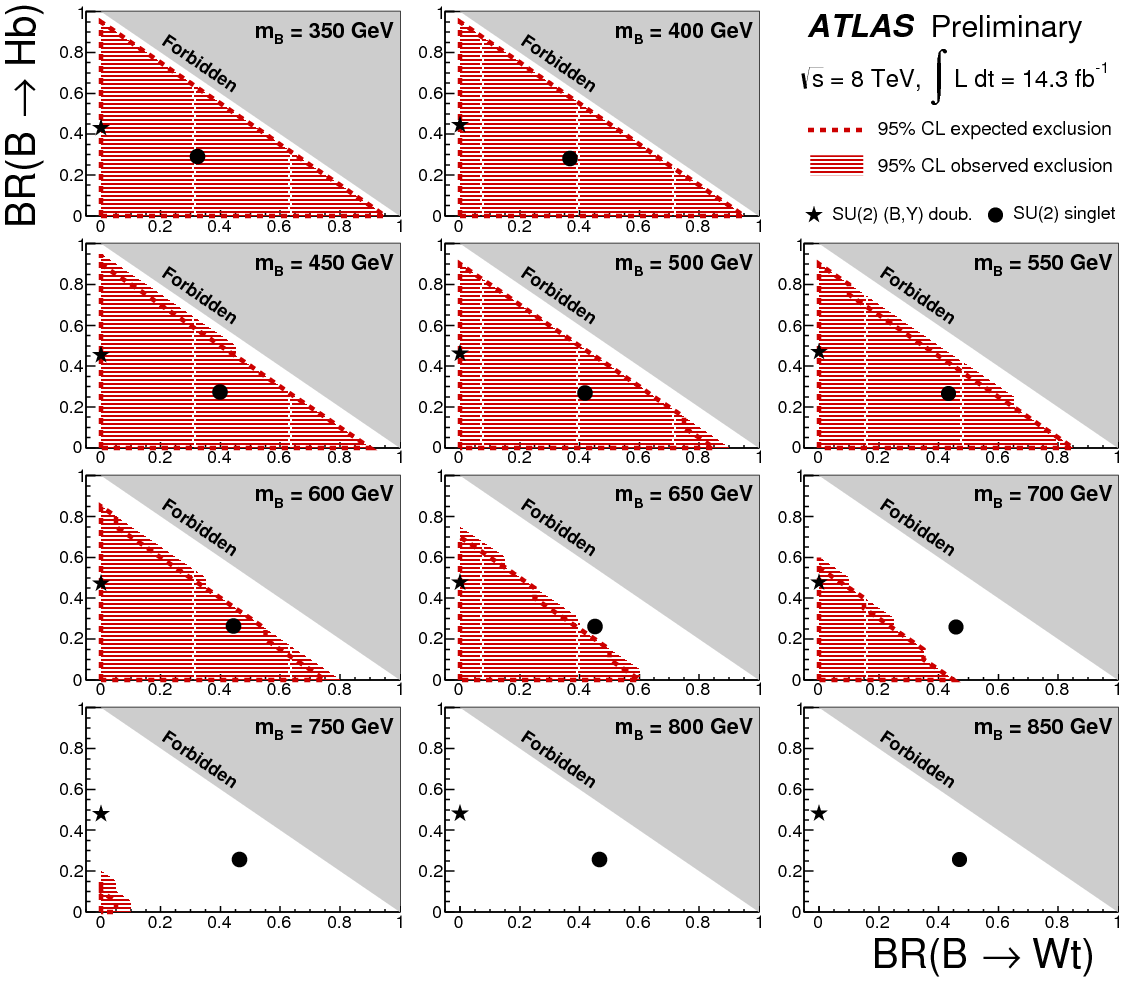
\includegraphics[width=.7\textwidth]{pics/Tdilep/fig_10.png}

Limit setting:\\
binned maximum-likelihood ratio to fit $m_{Collinear}$\\
use the $CL_s$ technique (see e.g.~\cite{Junk:1999kv,Read:2002hq})\\

\vspace{\baselineskip}

setting an observed 95\% CL limit on fourth generation $t'$ mass at \alert{350~GeV}\\

\end{minipage}


\end{frame}


%%%%%%%%%%%%%%%%%%%%%%%%%%%%%%%%%%%%%%%%%%%%
%%%%%%%%%%%%%%%%%%%%%%%%%%%%%%%%%%%%%%%%%%%%
\section{Searches for Heavy Bottoms}
%%%%%%%%%%%%%%%%%%%%%%%%%%%%%%%%%%%%%%%%%%%%
%%%%%%%%%%%%%%%%%%%%%%%%%%%%%%%%%%%%%%%%%%%%
\begin{frame}\frametitle{SS Dilepton, 4.7\ifb~\cite{ATLAS-CONF-2012-130}} %({\small \href{https://cdsweb.cern.ch/record/1478217}{ATLAS-CONF-2012-130} \cite{ATLAS-CONF-2012-130}})}
\footnotesize\centering

\begin{minipage}{.5\textwidth}
\centering


Analysis sensitive to 
\scriptsize
\begin{itemize}
\item fourth generation $b'$
\item vector like quark $X(5/3)$
\item four tops
\end{itemize}

Final state has \alert{four $W$s} (two same sign $W$ for singly produced $X(5/3)$) $\rightarrow$ looking for two isolated \alert{same-sign leptons}
\begin{itemize}
\item Very few SM processes with such topology!
\item Main backgrounds: fakes and charge flips
\end{itemize}



\end{minipage}\begin{minipage}{.5\textwidth}
\centering

Additional analysis requirements

\scriptsize
\begin{itemize}
\item Two same charge leptons
\item At least two jets, at least one $b$tagged jet
\item Leading lepton $p_T>25$~GeV
\item same flavor: $m_{ll}>15~$GeV, \alert{$Z$ mass veto}
\item $\slashed{E}_T>40~$GeV
\item $H_T>550$~GeV
\end{itemize}

\end{minipage}

\vspace{\baselineskip}

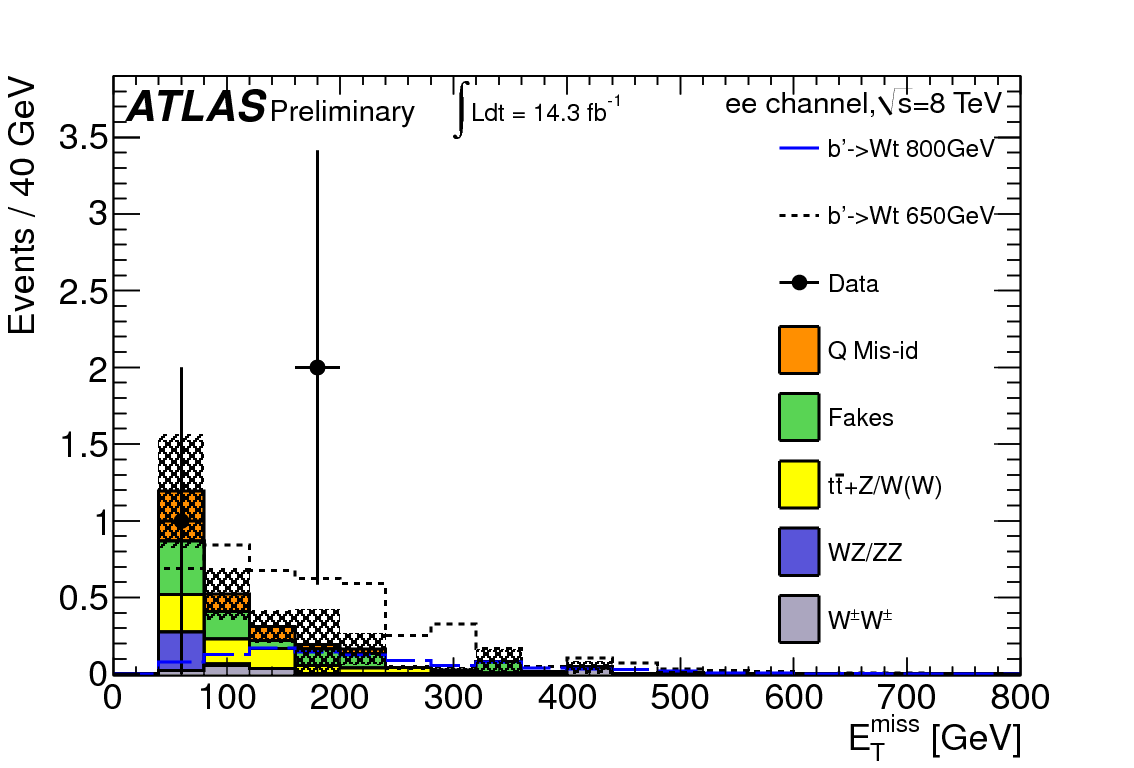
\includegraphics[width=.3\textwidth]{pics/Bdilep1/fig_03b.png}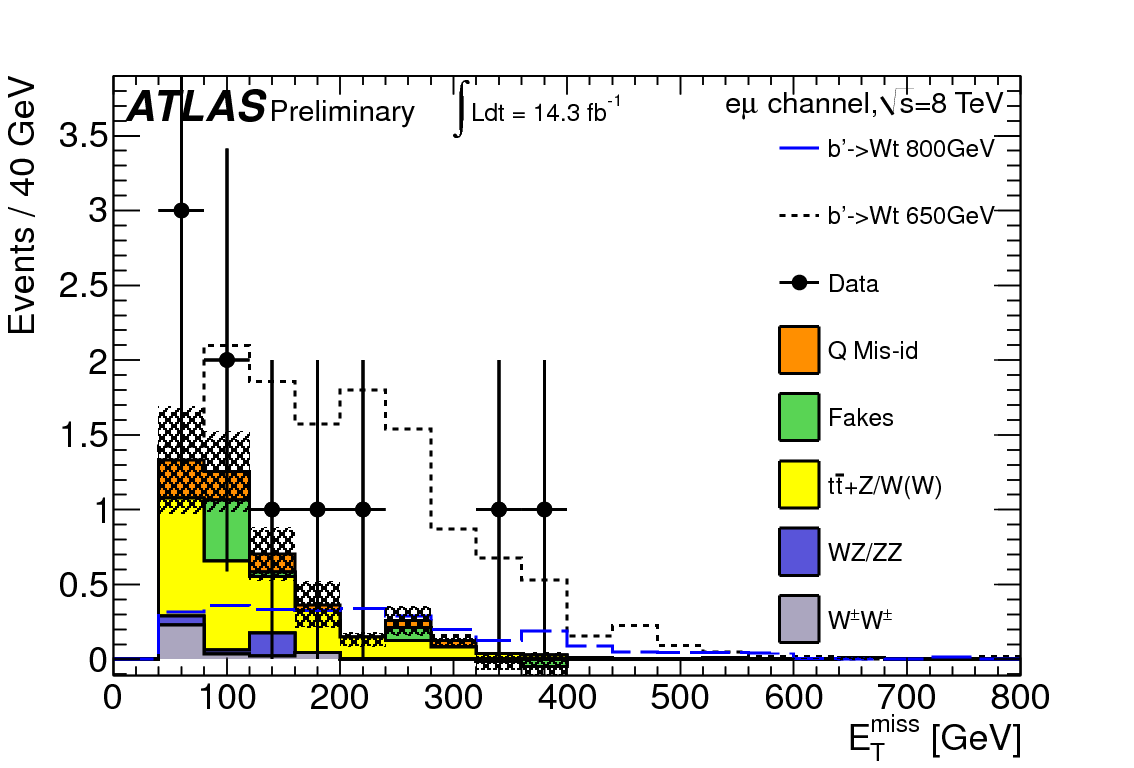
\includegraphics[width=.3\textwidth]{pics/Bdilep1/fig_03d.png}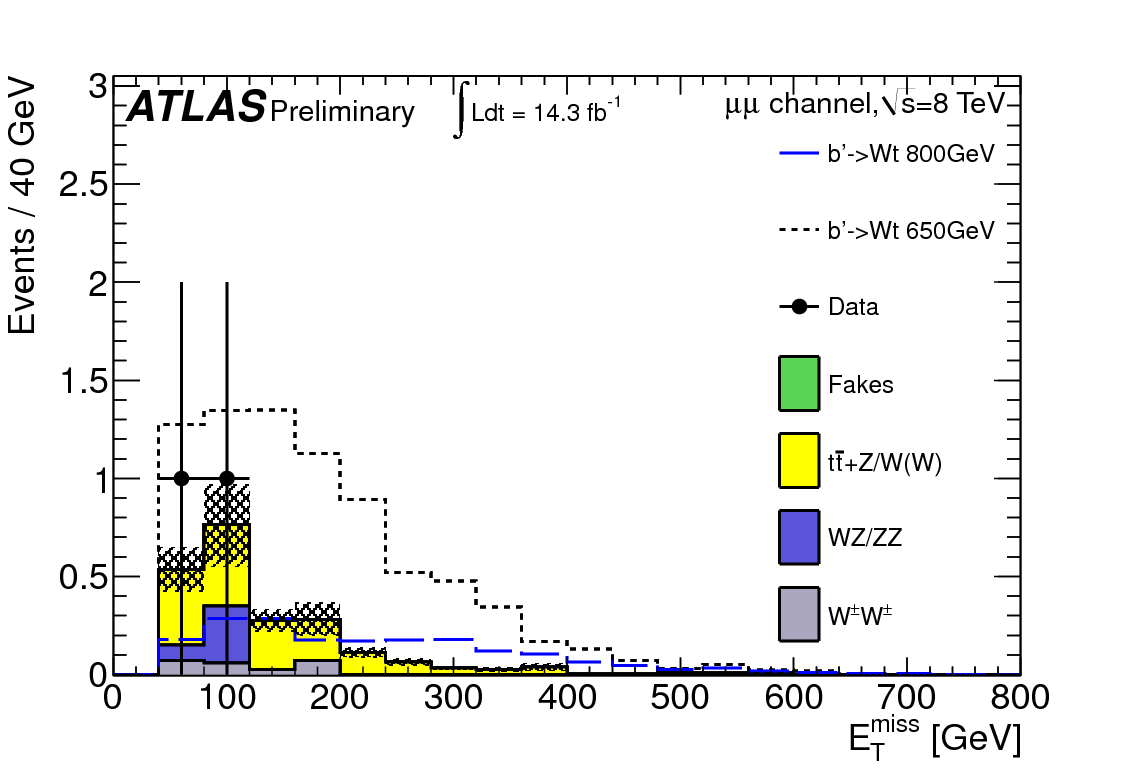
\includegraphics[width=.3\textwidth]{pics/Bdilep1/fig_03f.png}


\end{frame}



\begin{frame}\frametitle{SS Dilepton, 4.7\ifb~\cite{ATLAS-CONF-2012-130}} %({\small \href{https://cdsweb.cern.ch/record/1478217}{ATLAS-CONF-2012-130} \cite{ATLAS-CONF-2012-130}})}
\footnotesize\centering

\begin{minipage}{1.\textwidth}

\begin{minipage}{.5\textwidth}
\centering
\vspace{\baselineskip}

\includegraphics[width=.9\textwidth]{pics/Bdilep1/fig_04.png}

\end{minipage}\begin{minipage}{.5\textwidth}
\centering

Four events observed in signal region, 5.6$\pm$1.7 expected background\\

\vspace{\baselineskip}

Limit setting:\\
single bin counting experiment, using the $CL_s$ technique (see e.g. \cite{Junk:1999kv,Read:2002hq})\\
Excluded masses up to  \alert{670~GeV} at 95\% CL
\end{minipage}
\end{minipage}

\begin{minipage}{1.\textwidth}

\begin{minipage}{.5\textwidth}
\centering

$X(5/3)$ interpretation:\\
single production depends on the coupling constant $\lambda$ of the $tWX_{5/3}$ vertex
\begin{itemize}
\item studied $\lambda=1$, $\lambda=3$ and $\lambda << 1$
\end{itemize}
Not taken into account contribution from e.g. $T(2/3)$

\end{minipage}\begin{minipage}{.5\textwidth}
\centering

\vspace{-\baselineskip}
\vspace{-\baselineskip}
\vspace{-\baselineskip}

\includegraphics[width=.95\textwidth]{pics/Bdilep1/fig_05.png}

\end{minipage}
\vspace{-\baselineskip}
\centering
\scriptsize \hyperlink{Bdilep1}{more in Backup!}
\end{minipage}



\end{frame}


\begin{frame}\frametitle{OS Dilepton $Z$tag, 2.0\ifb~\cite{:2012aka}} %({\small \href{http://arxiv.org/abs/1204.1265}{arXiv:1204.1265} \cite{:2012aka}})}
\footnotesize\centering

\begin{minipage}{.5\textwidth}
\centering

Looking for an heavy \alert{$b'\rightarrow Zb$}\\
also sensitive to \alert{VLQ $B(-1/3)$}\\

\scriptsize 
\begin{itemize}
\item chiral $b'$: neutral-current mode occurs through \alert{loop diagrams} $\rightarrow$ if mass $>255~$GeV $b'\rightarrow Wt$ is favored
\item vector-like $B$: $B\rightarrow Zb$ is a \alert{tree level} process with B.R. comparable to the other two ($Wt, Hb$)
\end{itemize}

\alert{$b'$ candidate}: $e^+e^-$ and highest-$p_T$ $b$jet

\includegraphics[width=.8\textwidth]{pics/Bdilep2/fig_04.png}

\end{minipage}\begin{minipage}{.5\textwidth}
\centering

\includegraphics[width=.9\textwidth]{pics/Bdilep2/fig_02.png}


Additional analysis requirements

\scriptsize
\begin{itemize}
\item $Z\rightarrow e^+e^-$ final states \alert{only}
\item At least one $b$jet
\item $|m_{ee} - m_Z|<15~$GeV
\item $p_T(Zb)>150$~GeV
\end{itemize}

Focusing only on the $Zb$ reconstruction, not looking at the other $b'$ decay

\vspace{-\baselineskip}
\begin{flushright}\scriptsize \hyperlink{Bdilep2}{more in Backup!}\end{flushright}


\end{minipage}

\end{frame}

\begin{frame}\frametitle{OS Dilepton $Z$tag, 2.0\ifb~\cite{:2012aka}} %({\small \href{http://arxiv.org/abs/1204.1265}{arXiv:1204.1265} \cite{:2012aka}})}
\footnotesize\centering

\begin{minipage}{.4\textwidth}
\centering

defining $\beta = 2\times BR(b'\rightarrow Zb) - BR(b'\rightarrow Zb)^2$

\vspace{\baselineskip}

\scriptsize 
$\beta$ describes the \alert{fraction of signal events} with at least one $b'\rightarrow Zb$ decay as a function of the $BR$
\begin{itemize}
\item $\beta$ = 1 is equal to $BR(b'\rightarrow Zb) = 1$
\item for VLQ singlet $B(-1/3)$ $\beta$ varies with the mass: $m_B = 200-700~$GeV $\rightarrow$ $\beta=0.9-0.5$ 
\end{itemize}

\end{minipage}\begin{minipage}{.6\textwidth}
\centering

\includegraphics[width=.9\textwidth]{pics/Bdilep2/fig_05.png}
\end{minipage}

Limit setting:\\
using the $CL_s$ technique (see e.g. \cite{Junk:1999kv,Read:2002hq})\\

\vspace{\baselineskip}

VLQ $b'$ going 100\% to $Zb$ with $m_{b'}<$\alert{400~GeV} are excluded at 95\% CL\\
VLQ singlets $B(-1/3)$ with $m_B<$\alert{358~GeV} are excluded at 95\% CL\\

\end{frame}




\begin{frame}\frametitle{L+jets, 1.04\ifb~\cite{ATLAS:2012aw}} %({\small \href{http://arxiv.org/abs/1202.6540}{arXiv:1202.6540} \cite{ATLAS:2012aw}})}
\footnotesize\centering

\begin{minipage}{.35\textwidth}
\centering

Looking for \alert{$b'\rightarrow Wt$}\\
\scriptsize
assuming $m_{b'} > m_W + m_t$\\
and 100\% B.R.

\vspace{\baselineskip}
\vspace{\baselineskip}

\includegraphics[width=.9\textwidth]{pics/Bsinglelep/fig_04.png}

Nine exclusive bins in $(N_W, N_j)$

\end{minipage}\begin{minipage}{.65\textwidth}
\centering
\alert{Boosted topology}\\
\scriptsize
$\Delta R(j,j) \sim 2m_W/p_T^W$\\

\includegraphics[width=.5\textwidth]{pics/Bsinglelep/fig_03.png}\includegraphics[width=.5\textwidth]{pics/Bsinglelep/fig_02.png}


Additional analysis requirements

\scriptsize
\begin{itemize}
\item At least \alert{six jets}%, at least one $b$tagged jet
\end{itemize}
Reconstruct $W$ bosons as \alert{jet pairs} with $\Delta R<1.0$
\begin{itemize}
\item $N_W$ is the number of these jet pairs with mass in [70,100]~GeV
\end{itemize}

\end{minipage}

\begin{flushright}\scriptsize \hyperlink{Bsinglelep}{more in Backup!}\end{flushright}

\vspace{-\baselineskip}
\vspace{-\baselineskip}

\end{frame}


\begin{frame}\frametitle{L+jets, 1.04\ifb~\cite{ATLAS:2012aw}} %({\small \href{http://arxiv.org/abs/1202.6540}{arXiv:1202.6540} \cite{ATLAS:2012aw}})}
\footnotesize\centering

\begin{minipage}{.4\textwidth}
\centering


\scriptsize

Low $N_W$ and jet multiplicity bins are used to \alert{constrain} some systematic uncertainties

\includegraphics[width=.9\textwidth]{pics/Bsinglelep/fig_04mod.png}

Limit setting:\\
using the $CL_s$ technique (see e.g. \cite{Junk:1999kv,Read:2002hq})\\

\vspace{\baselineskip}

\end{minipage}\begin{minipage}{.6\textwidth}
\centering

\includegraphics[width=.9\textwidth]{pics/Bsinglelep/fig_05.png}

Masses below \alert{480~GeV} are excluded at 95\%

\end{minipage}

\end{frame}


\begin{frame}\frametitle{Single Production, 4.64\ifb~\cite{ATLAS-CONF-2012-137}} %({\small \href{http://cdsweb.cern.ch/record/1480628}{ATLAS-CONF-2012-137} \cite{ATLAS-CONF-2012-137}})}
\footnotesize\centering

\begin{minipage}{.4\textwidth}
\centering
\alert{Single production} of VLQ doublets with vector like quarks $U(+2/3)$, $D(-1/3)$, $X(+5/3)$\\
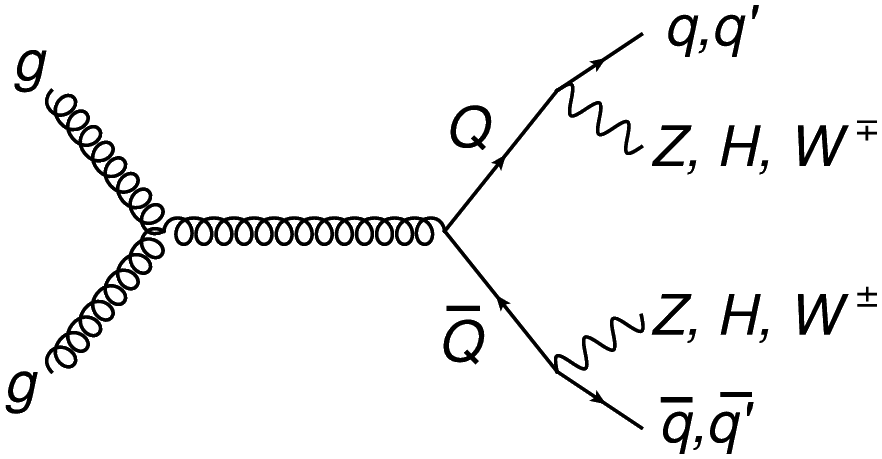
\includegraphics[width=.5\textwidth]{pics/Bsingleprod/fig_01a.png}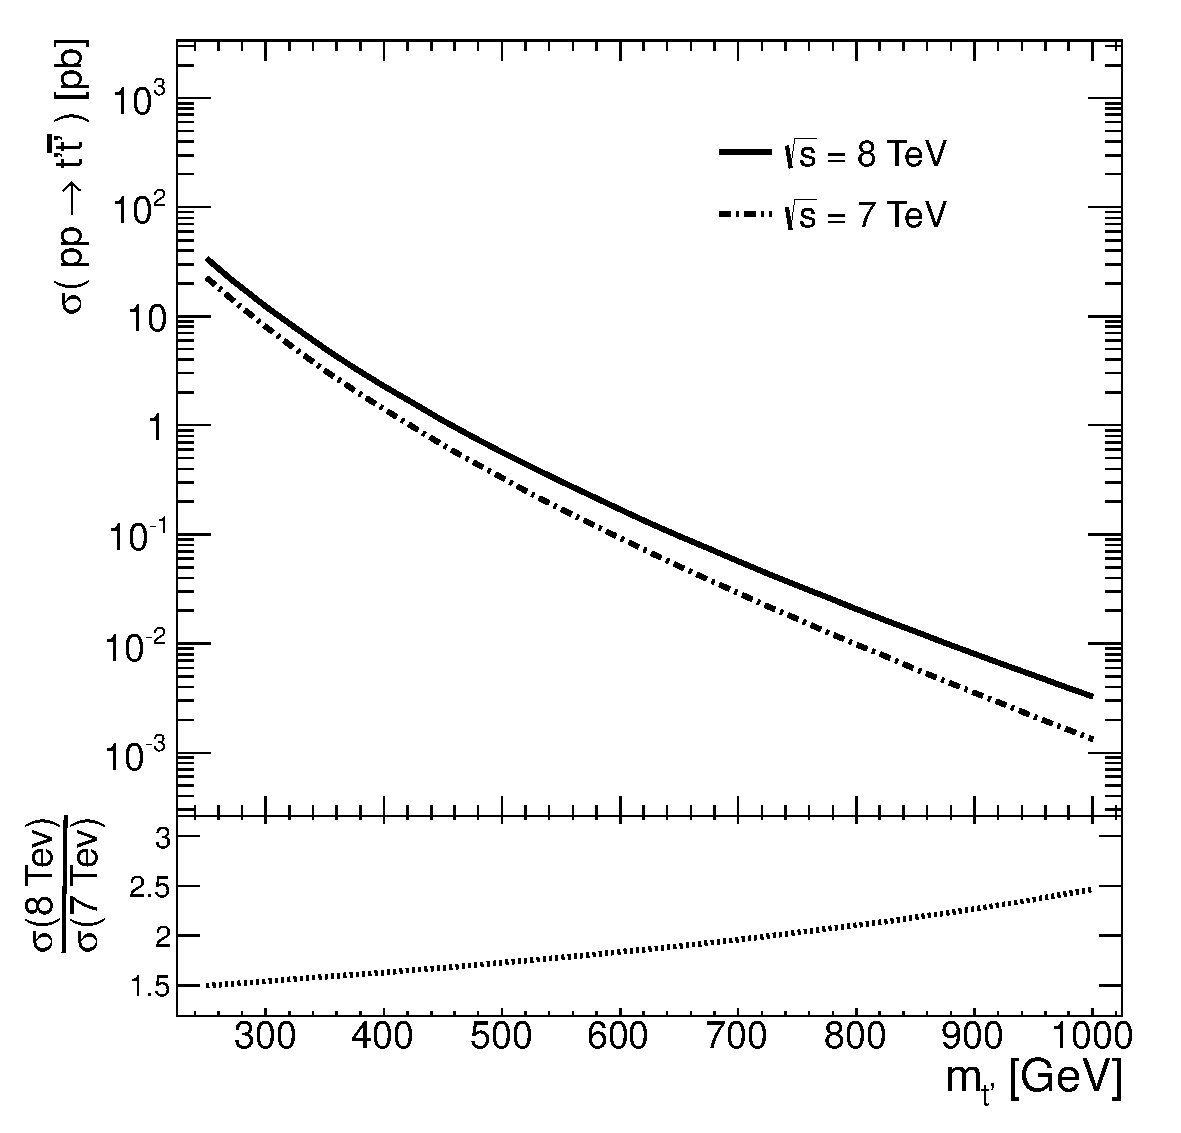
\includegraphics[width=.4\textwidth]{pics/Bsingleprod/fig_01b.png}
\scriptsize

Assumptions
\begin{itemize}
\item VLQs couple mainly to \alert{first generation} quarks
\item \alert{effective coupling} $k_{qQ} = (v/m_Q)\tilde{k}_{qQ}$ ($v$ Higgs vacuum expectation value, $\tilde{k}_{qQ}$ model-dependent parameter of $\mathcal{O}(1)$)
\end{itemize}

Signatures
\begin{itemize}
\item \alert{Charged Current (CC)}: $D\rightarrow Wu$, $X\rightarrow Wu$
\item \alert{Neutral Current (NC)}: $U\rightarrow Zu$
\end{itemize}

\end{minipage}\begin{minipage}{.6\textwidth}
\centering

Additional Analysis requirements

\renewcommand{\tabcolsep}{-0.1cm}
{\scriptsize
\begin{tabular}{p{0.5\textwidth}p{0.5\textwidth}}
CC Channel: & NC Channel: \\
\begin{itemize}
\item Exactly \alert{one} lepton
\item $\slashed{E}_T>50$~GeV
\item $m_T(W)>40~$GeV, $\eta(W)<2.5$
\item leading jet $p_T>60~$GeV
\item at least two jets
\end{itemize} & 
\begin{itemize}
\item Two same flavor, \alert{opposite charge} leptons
\item $m_{ll}$ in [66,116]~GeV
\item at least two jets
\end{itemize} \\
\end{tabular}
}


Cut optimizations through TMVA~\cite{2007physics...3039H}
{\scriptsize
\begin{tabular}{p{0.5\textwidth}p{0.5\textwidth}}
\begin{itemize}
\item $|\Delta \eta(W,$lead jet$)|<$2.3
\item $|\Delta \phi(W,$lead jet$)|>$ 2.1~rad
\item $|\Delta \phi(l,\slashed{E}_T)|<$ 1.3~rad
\item $|\Delta \eta(W,$ass jet$)|>$1.6
\item $|\Delta \eta($lead jet, ass jet$)|>$1.3
\end{itemize} & {\hspace{-2cm}
\begin{itemize}
\item $|\Delta \phi(l,l)|<$1.5~rad
\item $|\Delta \eta(l,l)|<$1.6
\item $|\Delta \phi(Z,$lead jet$)|>$ 2.1~rad
\item $|\Delta \eta(Z,$lead jet$)|<$1.1
\item $|\Delta \eta(Z,$ass jet$)|>$0.9
\item $|\Delta \eta($lead jet, ass jet$)|>$0.9
\end{itemize} }\\
\end{tabular}
}

\end{minipage}

\end{frame}



\begin{frame}\frametitle{Single Production, 4.64\ifb~\cite{ATLAS-CONF-2012-137}} %({\small \href{http://cdsweb.cern.ch/record/1480628}{ATLAS-CONF-2012-137} \cite{ATLAS-CONF-2012-137}})}
\footnotesize\centering


Using the BumpHunter~\cite{2011arXiv1101.0390C} to find data excess over smooth background distributions\\

\begin{minipage}{1.\textwidth}
\begin{minipage}{.5\textwidth}\scriptsize\centering
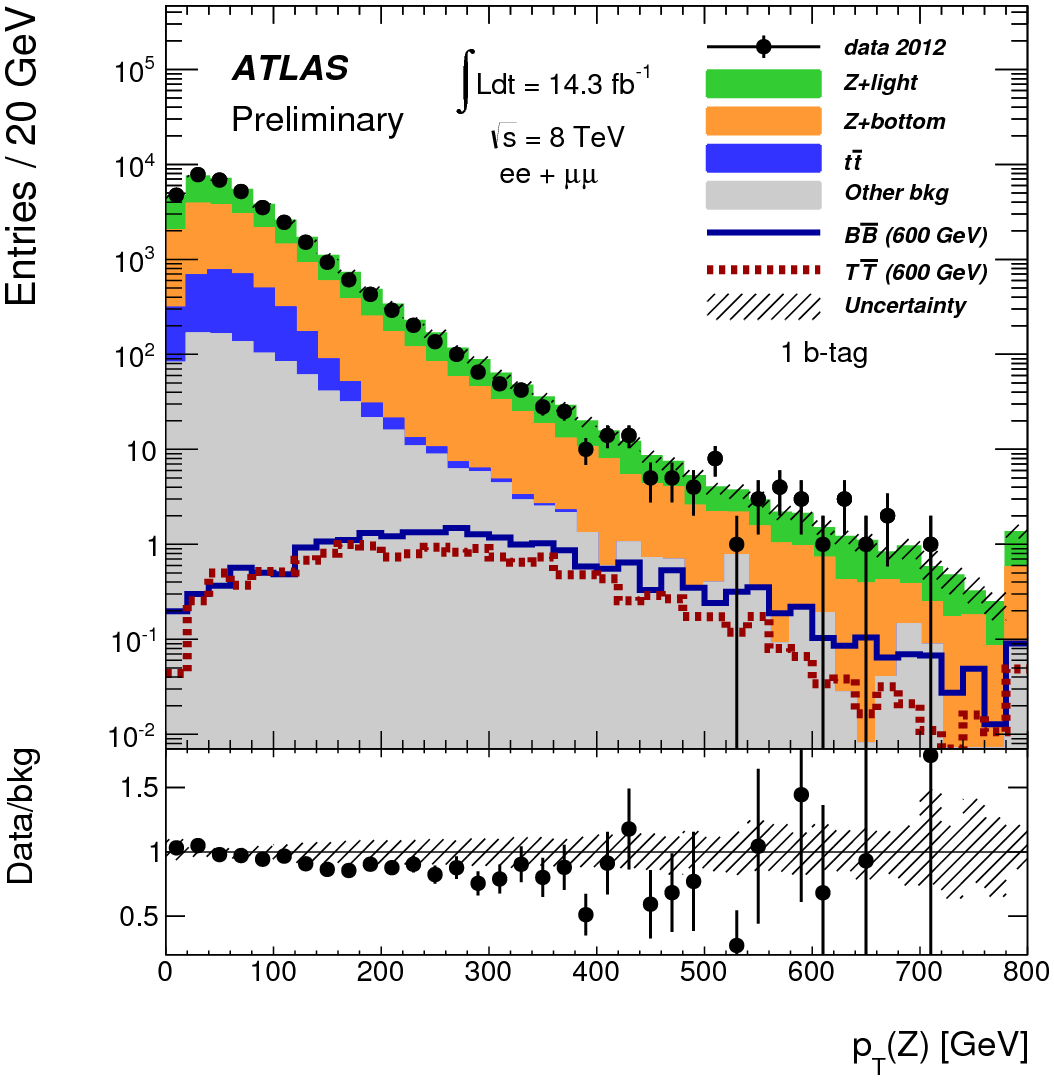
\includegraphics[width=.9\textwidth, height=.4\textheight]{pics/Bsingleprod/fig_05a.png}\\
\end{minipage}\begin{minipage}{.5\textwidth}\scriptsize\centering
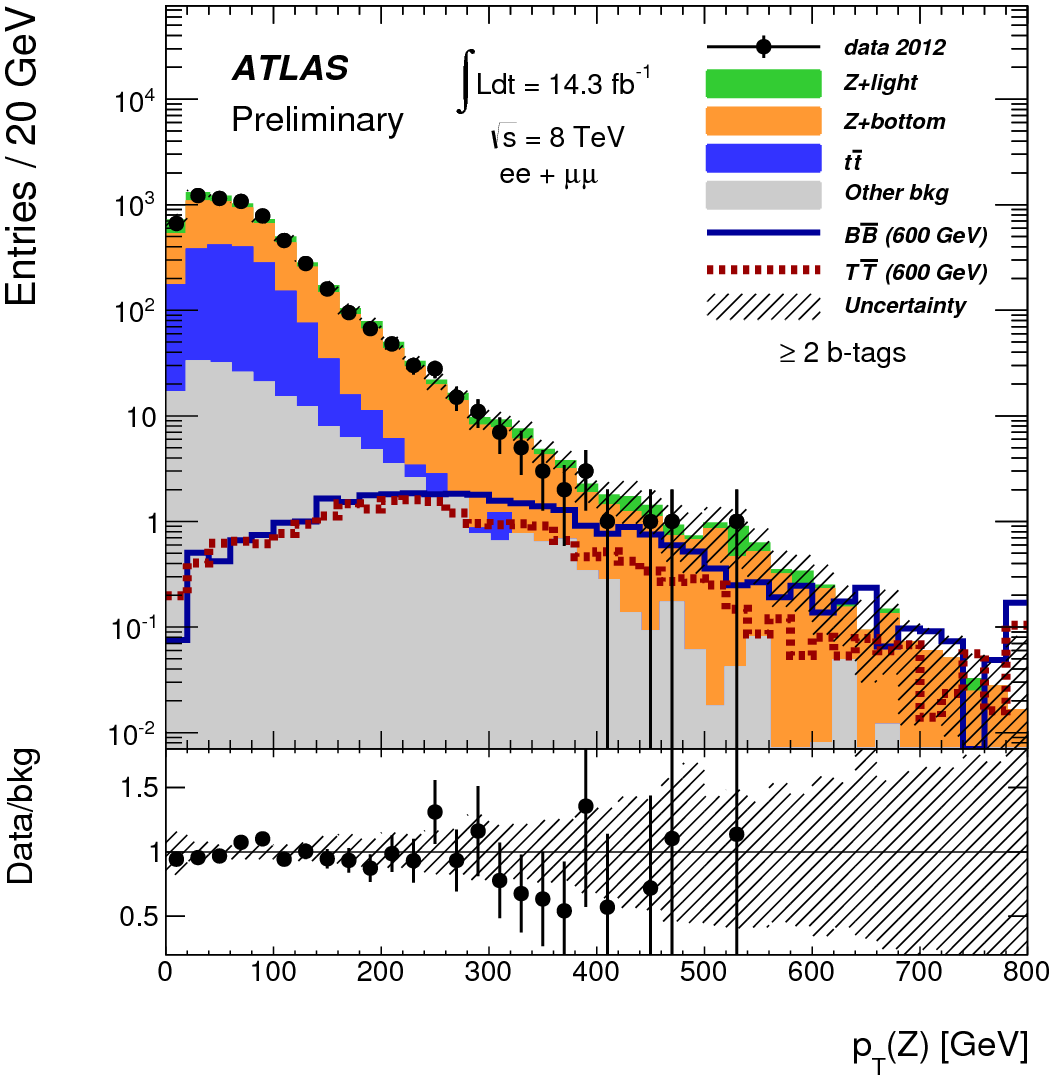
\includegraphics[width=.9\textwidth, height=.4\textheight]{pics/Bsingleprod/fig_05b.png}\\
\end{minipage}
\end{minipage}
\begin{minipage}{1.\textwidth}
\begin{minipage}{.5\textwidth}\scriptsize\centering

\vspace{\baselineskip}
\vspace{\baselineskip}
\vspace{\baselineskip}

Expected and observed 95\% C.L. upper limits on $\tilde{\kappa}^{2}_{qD}$, $\tilde{\kappa}^{2}_{qX}$, and $\tilde{\kappa}^{2}_{qU}$

\vspace{\baselineskip}
\vspace{\baselineskip}
\vspace{\baselineskip}

\hyperlink{Bsingleprod}{more in Backup!}

\end{minipage}\begin{minipage}{.5\textwidth}\scriptsize\centering
\includegraphics[width=.9\textwidth, height=.4\textheight]{pics/Bsingleprod/fig_05c.png}\\
\end{minipage}
\end{minipage}


\end{frame}




\section{Conclusions}

\begin{frame}\frametitle{Summary}
\footnotesize\centering



\begin{minipage}{.5\textwidth}
\centering
Searching for heavy quarks, ATLAS was able to set 95\% CL limits on various models:

\begin{itemize}[<+->]\scriptsize
\item[\cite{ATLAS:2012qe}] chiral 4th generation $t'$ (100\% to $Wb$) and  vector like $Y(-4/3)$: not below \alert{656~GeV}
\item[\cite{Aad:2012bt}] chiral 4th generation $t'$ (to $Wq$, $q=d,s,b$): not below \alert{350~GeV}
\item[\cite{ATLAS-CONF-2012-130}] chiral 4th generation $b'$ (100\% to $Wt$) and vector like $X(5/3)$: not below \alert{670~GeV}
\item[\cite{:2012aka}] vector like $b'$ (100\% to $Zb$): not below \alert{400~GeV}
\item[\cite{:2012aka}] vector like $B(-1/3)$ singlet: not below \alert{358~GeV}
\item[\cite{ATLAS:2012qe}] vector like $T(2/3)$: singlet model excluded up to \alert{500~GeV}
%\item vector like $X(5/3)$: not below~GeV
%\item vector like $Y(-4/3)$: not below~GeV
%\item singly produced vector like $U(2/3)$, $X(5/3)$, $D(-1/3)$: not below \alert{1080, 1420, 1120~GeV} respectively
\item[\cite{ATLAS-CONF-2012-137}] vector like $U(2/3)$, $X(5/3)$, $D(-1/3)$: set limits as a function of mixing with first generation
\end{itemize}

\pause
\dots using only 2011 data!

\end{minipage}\begin{minipage}{.5\textwidth}
\centering
\pause
2012 run at $\sqrt{s}=8~$TeV, more than 20\ifb collected!\\{\scriptsize And VLQ \hyperlink{vlqXsec}{production cross sections} significantly increase!}

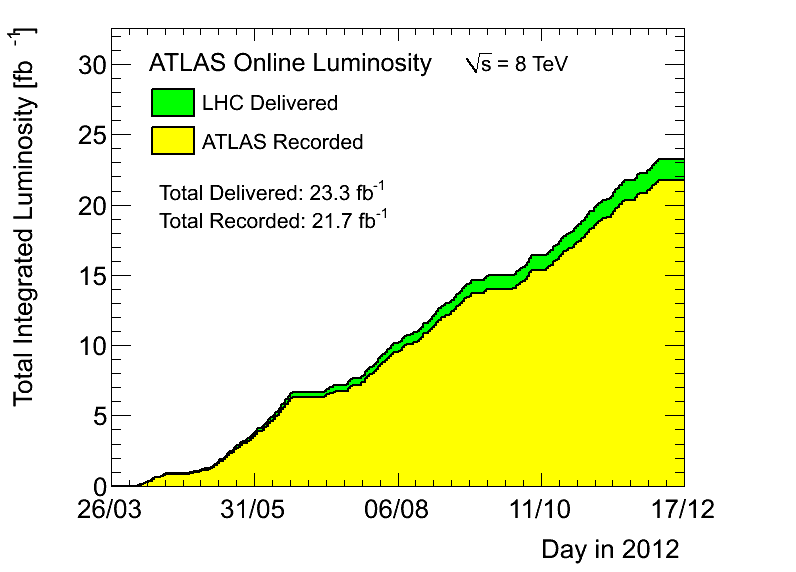
\includegraphics[width=.9\textwidth,height=.35\textheight]{pics/sumLumiByDay2012}

so maybe we'll be able to say:

\pause
\begin{minipage}{.1\textwidth}
\phantom{aaaaaa}
\end{minipage}\begin{minipage}{.9\textwidth}
\begin{beamercolorbox}[wd=.9\textwidth,rounded=true,shadow=true]{boxcolor}%structure!70!white}
\begin{quote}
I've seen things you people wouldn't believe\dots

\vspace{\baselineskip}

\hfill \tiny [Roy Batty,  Blade Runner (1982)]
\end{quote}
\end{beamercolorbox}
\end{minipage}

\end{minipage}

\end{frame}



\appendix


\section*{References}
\setbeamertemplate{bibliography item}[text]

\begin{frame}[allowframebreaks]
\frametitle{References}\footnotesize
%\bibliographystyle{apalike}
%\bibliographystyle{phjcp}
%\bibliographystyle{acm}
\bibliographystyle{myunsrt}
%\bibliographystyle{plain}
%\bibliographystyle{REVTeX4.1}
\bibliography{bib_files/heavyquarks.bib}
\end{frame}


\section*{Backup}

%----------------------------------
\begin{frame}
 \frametitle{}

\begin{center}{\bfseries
BACKUP SLIDES}
\end{center}
\end{frame}


\begin{frame}[label=vlqBR]\frametitle{Vector Like Quarks B.R.s \cite{Martin:2009bg}}
\footnotesize\centering

Brancing Ratios for the $T(2/3)$ vector like quark

\begin{minipage}{.5\textwidth}
\centering
``Democratic''
\end{minipage}\begin{minipage}{.5\textwidth}
\centering
``W-phobic''
\end{minipage}

\includegraphics[width=.9\textwidth]{pics/BRvlq.png}

\end{frame}


\begin{frame}[label=vlqXsec]\frametitle{Vector Like Quarks Pair Production Xsec}
\footnotesize\centering

NNLO $Q\bar{Q}$ production cross sections from \href{https://twiki.cern.ch/twiki/bin/view/Sandbox/CrossSectionsCalculationTool}{HATHOR} for $pp$ collision at LHC 
center of mass energies of 7~TeV and 8~TeV

\includegraphics[width=.5\textwidth]{pics/xsecvlq.png}

\end{frame}



\begin{frame}[label=Tsinglelep]\frametitle{L+jets, 4.7~fb$^{-1}$ ({\small \href{http://arxiv.org/abs/1210.5468}{arXiv:1210.5468} \cite{ATLAS:2012qe}})} 
\footnotesize\centering


\begin{minipage}{.35\textwidth}
\centering 

\textit{tight} isolation requirements

\scriptsize
\begin{itemize}
\item $min(\Delta R(l,b_{1,2})) > 1.4$
\end{itemize}

\includegraphics[width=.9\textwidth,height=.3\textheight]{pics/Tsinglelep/figaux_09.png}

\begin{itemize}
\item $min(\Delta R(W_{had},b_{1,2})) > 1.4$
\end{itemize}
\includegraphics[width=.9\textwidth,height=.3\textheight]{pics/Tsinglelep/figaux_10.png}

{\tiny (distributions after loose selection, except for boosted condition $\Delta R(l,\nu)<1.4$)}

\end{minipage}\begin{minipage}{.65\textwidth}
\centering

\includegraphics[width=.5\textwidth]{pics/Tsinglelep/fig_02a.png}
\includegraphics[width=.5\textwidth]{pics/Tsinglelep/fig_02b.png}

\textit{loose} and \textit{tight} mass reconstruction

\end{minipage}


\end{frame}


\begin{frame}[label=Tdilep]\frametitle{OS Dilepton, 1.04~fb$^{-1}$ ({\small \href{http://arxiv.org/abs/1202.3389}{arXiv:1202.3389} \cite{Aad:2012bt}})}
\footnotesize\centering


\begin{minipage}{.35\textwidth}
\centering

Additional cuts for $t\bar{t}$ discrimination
\vspace{\baselineskip}


\includegraphics[width=.9\textwidth]{pics/Tdilep/figaux_12a.png}\\
\includegraphics[width=.9\textwidth]{pics/Tdilep/figaux_12b.png}

\end{minipage}\begin{minipage}{.65\textwidth}
\centering
\includegraphics[width=.5\textwidth]{pics/Tdilep/tab1}\includegraphics[width=.5\textwidth]{pics/Tdilep/tab2}\\

$m_{Collinear}$ reconstruction:

\begin{itemize}
\item Reconstruct the two neutrinos assuming only contribution from $\slashed{E}_T$
\item Consider as free parameters in [0,1] $|\Delta\eta(l,\nu)|$ and $|\Delta\phi(l,\nu)|$
\item Set them as the values that with jet assignment minimizes the differences between the two masses
\end{itemize}
\end{minipage}


\end{frame}


\begin{frame}[label=Bdilep1]\frametitle{SS Dilepton, 4.7\ifb ({\small \href{https://cdsweb.cern.ch/record/1478217}{ATLAS-CONF-2012-130} \cite{ATLAS-CONF-2012-130}})}
\footnotesize\centering

Observed and expected number of events in the signal region\\
Errors are stat and syst respectively

\includegraphics[width=.9\textwidth]{pics/Bdilep1/tab2}

\end{frame}


\begin{frame}\frametitle{SS Dilepton, 4.7\ifb ({\small \href{https://cdsweb.cern.ch/record/1478217}{ATLAS-CONF-2012-130} \cite{ATLAS-CONF-2012-130}})}
\footnotesize\centering

Expected and observed limits on the masses of the three considered signals

\includegraphics[width=.8\textwidth]{pics/Bdilep1/tab1}

\end{frame}


\begin{frame}[label=Bdilep2]\frametitle{OS Dilepton $Z$tag, 2.0\ifb ({\small \href{http://arxiv.org/abs/1204.1265}{arXiv:1204.1265} \cite{:2012aka}})}
\footnotesize\centering


\begin{minipage}{.5\textwidth}
\centering
$\geq 1 $ jet\\
\includegraphics[width=.8\textwidth]{pics/Bdilep2/fig_01}
\end{minipage}\begin{minipage}{.5\textwidth}
\centering
$\geq 1$ $b$jet\\
\includegraphics[width=.8\textwidth]{pics/Bdilep2/fig_02}
\end{minipage}

both before the $Z$ mass window cut

\end{frame}


\begin{frame}[label=Bsinglelep]\frametitle{L+jets, 1.04\ifb ({\small \href{http://arxiv.org/abs/1202.6540}{arXiv:1202.6540} \cite{ATLAS:2012aw}})}
\footnotesize\centering

\begin{minipage}{.5\textwidth}
Number of events in $(N_W, N_j)$ bins\\
\includegraphics[width=.8\textwidth]{pics/Bsinglelep/tab1}
\end{minipage}\begin{minipage}{.5\textwidth}
Systematics\\
\includegraphics[width=.8\textwidth]{pics/Bsinglelep/tab2}
\end{minipage}

\end{frame}


\begin{frame}[label=Bsingleprod]\frametitle{Single Production, 4.64\ifb ({\small \href{http://cdsweb.cern.ch/record/1480628}{ATLAS-CONF-2012-137} \cite{ATLAS-CONF-2012-137}})}
\footnotesize\centering


Using the BumpHunter~\cite{2011arXiv1101.0390C} to find data excess over smooth background distributions\\

\begin{minipage}{.5\textwidth}\scriptsize\centering
\includegraphics[width=.75\textwidth, height=.4\textheight]{pics/Bsingleprod/fig_03a.png}\\
\includegraphics[width=.9\textwidth, height=.4\textheight]{pics/Bsingleprod/fig_04a.png}\\
no $X(5/3)$, $D(-1/3)$ up to \alert{1420, 1120~GeV}
\end{minipage}\begin{minipage}{.5\textwidth}\scriptsize\centering
\includegraphics[width=.75\textwidth, height=.4\textheight]{pics/Bsingleprod/fig_03b.png}\\
\includegraphics[width=.9\textwidth, height=.4\textheight]{pics/Bsingleprod/fig_04b.png}\\
no $U(2/3)$ up to \alert{1080~GeV}
\end{minipage}


\end{frame}

\end{document}
